\documentclass[12pt]{article}

% Packages
\usepackage[margin=1.2in]{geometry}
\usepackage{graphicx}
\usepackage{enumerate}
\usepackage{listings}
\usepackage{titling}
\usepackage{tabularx}
\usepackage{longtable}
\usepackage{booktabs}
\usepackage{hyperref}
\usepackage{makecell}
\usepackage{caption}
\usepackage{array}
\lstset{basicstyle=\small\ttfamily,xleftmargin=18pt,breaklines=true}
\captionsetup[table]{skip=2pt}
% Comments --------------------------------------------------------------------
\usepackage{xcolor}
\newif\ifcomments\commentsfalse
\ifcomments \newcommand{\authornote}[3]{\textcolor{#1}{[#3 ---#2]}}
\newcommand{\todo}[1]{\textcolor{red}{[TODO: #1]}} \else
\newcommand{\authornote}[3]{} \newcommand{\todo}[1]{} \fi
\newcommand{\wss}[1]{\authornote{magenta}{SS}{#1}}
\newcommand{\ds}[1]{\authornote{blue}{DS}{#1}}
\newcommand{\sd}[1]{\authornote{green}{SD}{#1}}
\newcommand{\mmp}[1]{\authornote{green}{MP}{#1}}
% End Comments ---------------------------------------------------------------

\setlength\parindent{0pt} % Cleaner look


\usepackage{xcolor}
\hypersetup{
    colorlinks,
    linkcolor={red!50!black},
    citecolor={blue!50!black},
    urlcolor={blue!80!black}
}

% Title Page -----------------------------------------------------------------
\title{
\LARGE GEANT4-GPU:
\\\vspace{10mm}
\large \textbf{User Manual}
\vspace{40mm}
}
\author{
Stuart Douglas -- dougls2
\\Matthew Pagnan -- pagnanmm
\\Rob Gorrie -- gorrierw
\\Victor Reginato -- reginavp
\vspace{10mm}
}
\date{\vfill \textbf{Version 1}\\ \today}
% End Title Page -------------------------------------------------------------

% ============================== BEGIN DOCUMENT ============================= %
\begin{document}
\pagenumbering{gobble} % start numbering after TOC

% ============================== Title Page ============================= %
\maketitle
\newpage

% ================================= TOC ================================= %
\newgeometry{bottom=1.1in, top=1.1in}
\tableofcontents
\newpage
\pagenumbering{arabic}
\restoregeometry

% =============================== Section =============================== %
\section{Revision History}
All major edits to this document will be recorded in the table below.

\begin{table}[h]
\centering
\caption{Revision History}\label{Table_Revision}
\begin{tabular}{lll}
\toprule
\bf Description of Changes & \bf Author & \bf Date\\\midrule
Proper spelling of Geant4, & Stuart & 2016-04-24\\
Fixed links & Matt & 2016-03-07\\
Initial draft of document & Matt, Stuart, Rob, Victor  & 2016-02-26\\
\bottomrule
\end{tabular}
\end{table}

% =============================== Section =============================== %
\section{List of Figures}
GEANT4-GPU is a command-line driven program, so only a few figures are included. Commands and results are kept in-line within the text, formatted using a \texttt{monospace} typeface.

\begin{table}[h]
\centering
\caption{List of Figures}
\begin{tabular}{ll}
\toprule
\textbf{Figure \#} & \textbf{Description}\\\midrule
\ref{FigCmake} & Results of running original CMake command to generate build files\\
\ref{FigDisable} & Results of running CMake command to disable CUDA acceleration\\
\ref{FigVis} & Visualization of Hadr04 example in Geant4\\
\bottomrule
\end{tabular}
\end{table}

\ds{You should consider adding some figures (even just screenshots of console results)
	to add some variety to the document. It makes it easier to read.}
\sd{Added some figures}

\section{Definitions and Acronyms} % Matt
\begin{table}[h]
\centering
\caption{Definitions and Acronyms}
\begin{tabularx}{\textwidth}{lX}
\toprule
\bf Term & \bf Description\\\midrule
Geant4 & Open-source software toolkit used to simulate the passage of particles through matter\\
GEANT4-GPU & Geant4 with some computations running on the GPU\\
GPU & Graphics processing unit, well-suited to parallel computing tasks\\
CPU & Computer processing unit, general computer processor well-suited to serial tasks\\
CUDA & Parallel computing architecture for general purpose programming on GPU, developed by NVIDIA\\
RHEL & Red Hat Enterprise Linux Server\\
OS X & Operating system developed by Apple\\
\Xhline{2\arrayrulewidth}
\end{tabularx}
\end{table}


% =============================== Section =============================== %

\section{Introduction} % Rob
\subsection{Purpose of Document} % Rob
The following user manual corresponds to the McMaster GEANT4-GPU project. The project, under the supervision of Dr. Emil Sekerinski and Dr. Adriaan Buijs, is a modification of the existing Geant4 codebase to leverage GPU computing in certain Geant4 modules. Geant4 is a software toolkit for developing particle simulations.\\

The main priority of this document is to provide users with all the information needed to install, run, and understand at a high level the GEANT4-GPU project. This includes the license, installation instructions, execution instructions, high-level overview of how CUDA was integrated, and a troubleshooting section.

\subsection{Background} % Rob
There have been several documented attempts in porting parts of Geant4 to the GPU prior to this project. None of these instances approach or discuss the problem in the same modularized fashion.\\

Alongside niche implementations specifically for medical applications (Bert J, Perez-Ponce H, Lemarchal Y, Gaens M, amongst others) there have also been documented GPU ports of more general Geant4 components (Otto Seiskarim Jukka Kommerim Tapio Niemi).\\

For background information regarding Geant4, refer to \ref{SecBackground}.

\subsection{Scope of Document} % Rob
The manual is intended to give basic insight into the nature of GEANT4-GPU and rigorous instructions on how to install and run the project. This document also includes a section for users who wish to integrate CUDA with other aspects of Geant4 in section \ref{SecDev}.\\

This document does not include information on how to use Geant4, or how to develop Geant4 simulations for particular problem domains.\\

A basic knowledge of programming concepts and command-line tools is assumed, as well as familiarity with Geant4.

\subsection{Document Overview} % Matt
This document first declares the legal information related to the use of the project. Following this are detailed step-by-step instructions on how to install the software. A section on creating and running simulations using the CUDA functionality introduced in GEANT4-GPU is then included. Following that is a section detailing high-level details about how the CUDA code was developed and integrated, guiding future developers on how to integrate CUDA into other parts of Geant4. A troubleshooting section is included as well as a FAQ section covering many common questions related to the project.

\section{Legal Information}	% Victor
\emph{This product includes software developed by Members of the Geant4 Collaboration (http://cern.ch/Geant4).}

\subsection{Geant4 Software License}
\begin{lstlisting}
Geant4 Software License
Version 1.0,  28 June 2006
 
Copyright (c) Copyright Holders of the Geant4 Collaboration, 1994-2006.
See http://cern.ch/Geant4/license for details on the copyright holders. All rights not expressly granted under this license are reserved.

This software includes voluntary contributions made to Geant4. See http://cern.ch/Geant4 for more information on Geant4.

Installation, use, reproduction, display, modification and redistribution of this software, with or without modification, in source and binary forms, are permitted on a non- exclusive basis. Any exercise of rights by you under this license is subject to the following conditions:

1. Redistributions of this software, in whole or in part, with or without modification, must reproduce the above copyright notice and these license conditions in this software, the user documentation and any other materials provided with the redistributed software.

2. The user documentation, if any, included with a redistribution, must include the following notice:
"This product includes software developed by Members of the Geant4 Collaboration ( http://cern.ch/Geant4 )."

If that is where third-party acknowledgments normally appear, this acknowledgment must be reproduced in the modified version of this software itself.

3. The names "Geant4" and "The Geant4 toolkit" may not be used to endorse or promote software, or products derived therefrom, except with prior written permission by license@Geant4.org. If this software is redistributed in modified form, the name and reference of the modified version must be clearly distinguishable from that of this software.

4. You are under no obligation to provide anyone with any modifications of this software that you may develop, including but not limited to bug fixes, patches, upgrades or other enhancements or derivatives of the features, functionality or performance of this software. However, if you publish or distribute your modifications without contemporaneously requiring users to enter into a separate written license agreement, then you are deemed to have granted all Members and all Copyright Holders of the Geant4 Collaboration a license to your modifications, including modifications protected by any patent owned by you, under the conditions of this license.

5. You may not include this software in whole or in part in any patent or patent application in respect of any modification of this software developed by you.

6. DISCLAIMER
THIS SOFTWARE IS PROVIDED BY THE MEMBERS AND COPYRIGHT HOLDERS OF THE Geant4 COLLABORATION AND CONTRIBUTORS "AS IS" AND ANY EXPRESS OR IMPLIED WARRANTIES, INCLUDING, BUT NOT LIMITED TO, IMPLIED WARRANTIES OF MERCHANTABILITY, OF SATISFACTORY QUALITY, AND FITNESS FOR A PARTICULAR PURPOSE OR USE ARE DISCLAIMED. THE MEMBERS OF THE Geant4 COLLABORATION AND CONTRIBUTORS MAKE NO REPRESENTATION THAT THE SOFTWARE AND MODIFICATIONS THEREOF, WILL NOT INFRINGE ANY PATENT, COPYRIGHT, TRADE SECRET OR OTHER PROPRIETARY RIGHT.

7. LIMITATION OF LIABILITY

THE MEMBERS AND COPYRIGHT HOLDERS OF THE Geant4 COLLABORATION AND CONTRIBUTORS SHALL HAVE NO LIABILITY FOR DIRECT, INDIRECT, SPECIAL, INCIDENTAL, CONSEQUENTIAL, EXEMPLARY, OR PUNITIVE DAMAGES OF ANY CHARACTER INCLUDING, WITHOUT LIMITATION, PROCUREMENT OF SUBSTITUTE GOODS OR SERVICES, LOSS OF USE, DATA OR PROFITS, OR BUSINESS INTERRUPTION, HOWEVER CAUSED AND ON ANY THEORY OF CONTRACT, WARRANTY, TORT (INCLUDING NEGLIGENCE), PRODUCT LIABILITY OR OTHERWISE, ARISING IN ANY WAY OUT OF THE USE OF THIS SOFTWARE, EVEN IF ADVISED OF THE POSSIBILITY OF SUCH DAMAGES.

8. This license shall terminate with immediate effect and without notice if you fail to comply with any of the terms of this license, or if you institute litigation against any Member or Copyright Holder of the Geant4 Collaboration with regard to this software.
\end{lstlisting}
 
\section{Installation} % Victor

\subsection{Supported Operating Systems} % Victor
GEANT4-GPU has been tested on OS X 10.11 and Red Hat Enterprise Linux Server release 6.7 (Santiago), henceforth called RHEL. Other versions of these operating systems are likely to work, but compatibility is not guaranteed.\\

To check what version of OS X you have, perform the following actions:

\begin{enumerate}
\item Click on the apple icon in the top left-hand corner of your screen.
\item Click on About This Mac.
\item Check to ensure that the version of your OS is 10.11 (El Capitan) (other versions may work, but are not guaranteed).
\end{enumerate}

To check your version of RHEL, perform the following actions:
\begin{enumerate}
\item Open a shell.
\item Type in the following command \texttt{cat /etc/redhat-release}
\item Check to ensure that the version of RHEL installed is 6.7 (Santiago) (other versions may work, but are not guaranteed).
\end{enumerate}

\subsection{Recommended Knowledge} % Victor
GEANT4-GPU is a scientific product for use in research. There is a large learning curve to using Geant4, and it is recommended that the user has familiarity with the following:
\begin{itemize}
\item Comfortable with the Unix command line. This includes navigating the file system, executing make files, and installing software through the command line.
\item Some knowledge of programming concepts and C++. Users develop their own simulations in C++ based off of the Geant4 toolkit, and as such some programming experience is recommended.
\item Understanding of physics concepts. The user is expected to be knowledgeable in their domain, as Geant4 requires an understanding of the physics processes in the simulation.
\end{itemize}

\subsection{Required Hardware} \label{SecCardReqs}% Victor
In order to successfully install and run Geant4 with GPU parallelism, you must first check that the workstation that you are installing on has a NVIDIA GPU with Compute Capability 3.0 or higher.\\

If the workstation does not have the requisite hardware, GEANT4-GPU may still be installed and executed with GPU computations disabled. In this case however, it is identical to the original Geant4 and it is recommended to use the official version from \url{http://cern.ch/geant4}.\\

To check if the GPU on your current workstation supports CUDA with a Compute Capability of 3.0 or higher, perform the following actions:\\

\begin{enumerate}
\item Determine the graphics card that is currently installed (RHEL)
\begin{enumerate}
\item Open a shell.
\item Enter the following command: \texttt{lspci | grep -i nvidia}
\item You should see output similar to the following:\\
\texttt{01:00.0 VGA compatible controller: NVIDIA Corporation GK104GL}\\
\texttt{[Quadro K5000] (rev a1)}
\item Where [\texttt{Quadro K5000}] is the name of your NVIDIA Graphics Card.
\end{enumerate}

\item Determine the graphics card that is currently installed (OS X)
\begin{enumerate}
\item Click on the apple icon in the top left-hand corner of your screen.
\item Click on About This Mac.
\item Click on More Info...
\item Under Contents click Hardware to view it's options.
\item Click on Graphics/Displays.
\item You should see the name of your card at the top of the right view-pane.
\end{enumerate}

\item Visit \url{https://developer.nvidia.com/cuda-gpus} and find your GPU to determine the Compute Capability of your card.
\item Check to ensure that you have a NVIDIA GPU with a  Compute Capability of at least 3.0.
\item If you can't find the currently installed GPU on the list, it is not CUDA compatible.
\end{enumerate}

\subsection{Required Software} % Victor
In order to install GEANT4-GPU you must have the following software installed:
\begin{itemize}
\item GCC version 4.9 (RHEL) or Clang version 6.0 or later (OS X). Note that McMaster's servers have GCC version 4.1, and an extra command is required to compile, as documented in section \ref{SecMac}.
\item CUDA Toolkit v6.5 (other versions may work, however 6.5 is the only one that is tested)
\item CMake 2.8 or higher
\end{itemize}

\subsubsection{Checking GCC Version (RHEL)}
\begin{enumerate}
\item Open a shell.
\item Enter \texttt{gcc -v} into the command line.
\item You will see output that looks like:
\texttt{gcc version 4.9.2 20150212 (Red Hat 4.9.2-6) (GCC)}
\item Ensure that the version number is 4.9
\end{enumerate}

\subsubsection{Checking Clang Version (OS X)}
\begin{enumerate}
\item Open a shell.
\item Enter \texttt{clang --version} into the command line.
\item You will see output similar to: \\
\texttt{Apple LLVM version 6.0 (clang-600.0.51) (based on LLVM 3.5svn)}\\
\texttt{Target: x86\_64-apple-darwin13.3.0}\\
\texttt{Thread model: posix}
\item Ensure that your version of Clang is at least \texttt{clang-600.x.xx}
\end{enumerate}

\subsubsection{CUDA Toolkit}
If you don't already have the CUDA Toolkit installed, visit \url{https://developer.nvidia.com/cuda-toolkit-65} and follow the installation instructions for your OS.\\

After installing, check to see that CUDA is up and running. For either RHEL or OS X:
\begin{enumerate}
\item Open a shell.
\item Enter the following command "nvcc --version"
\item Output should be similar to:\\
\texttt{nvcc: NVIDIA (R) Cuda compiler driver}\\
\texttt{Copyright (c) 2005-2014 NVIDIA Corporation}\\
\texttt{Built on Thu\_Jul\_17\_21:41:27\_CDT\_2014}\\
\texttt{Cuda compilation tools, release 6.5, V6.5.12}\\
\end{enumerate}

\subsubsection{CMake}
If you don't already have CMake (version 2.8 or higher) you can install it from: \url{https://CMake.org/download/}. After installing CMake, check to see that it is up and running. For either RHEL or OS X 10.11:
\begin{enumerate}
\item Open a shell.
\item Enter the following command: \texttt{CMake --version}.
\item Output should be similar to:\\
\texttt{CMake version 3.4.0}\\
\texttt{CMake suite maintained and supported by Kitware (kitware.com/CMake).}
\end{enumerate}

\subsection{Installation Instructions} % Victor
Included in the repository at \url{https://github.com/studouglas/GEANT4-GPU}, there is a README.md file that breaks down the installation steps, including special instructions on how to install this on McMaster's servers. That document is also covered in this section of the user guide.

\subsubsection{Installing GEANT4-GPU}
\begin{enumerate}
\item Clone the repository from \url{https://github.com/studouglas/GEANT4-GPU}
\item Open a shell
\item \label{StepMkdir} Navigate in the shell to the downloaded directory, and run the following command: \texttt{mkdir geant4.10.02-build geant4.10.02-install}
\item Navigate to the \texttt{geant4.10.02-build} directory you just created.
\item \label{StepCMake} Run the following command to start the build process:\\
\texttt{cmake -DGEANT4\_ENABLE\_CUDA=ON \textbackslash\\
 -DGEANT4\_USE\_SYSTEM\_EXPAT=OFF \textbackslash\\
 -DCMAKE\_INSTALL\_PREFIX=/path/to/GEANT4-GPU/geant4.10.02-install \textbackslash\\
 /path/to/GEANT4-GPU/geant4.10.02}
\begin{itemize}
\item \texttt{-DGEANT4\_ENABLE\_CUDA=ON} -- Setting this to \texttt{ON} will use your CUDA compiler to compile the CUDA code from the project and link it to the existing C++ code. Setting it to \texttt{OFF} (the default) will build Geant4 without any GPU functionality, and without requiring the CUDA compiler or a NVIDIA graphics card.
\item \texttt{-DGEANT4\_USE\_SYSTEM\_EXPAT=OFF} -- This simplifies the installation by using a version of the Expat library that is bundled with Geant4, rather than one that may or may not already be installed on the system. 
\item \texttt{-DCMAKE\_INSTALL\_PREFIX=...} -- Sets the directory to install all the compiled Geant4 libraries, datasets, and examples.
\end{itemize}
Note that running the above command for the first time can take several hours depending on your internet connection, as it must download large datasets required by Geant4.\\

\begin{figure}[!hbtp]
\caption{Output of CMake command in step \ref{StepCMake} on OS X}\label{FigCmake}
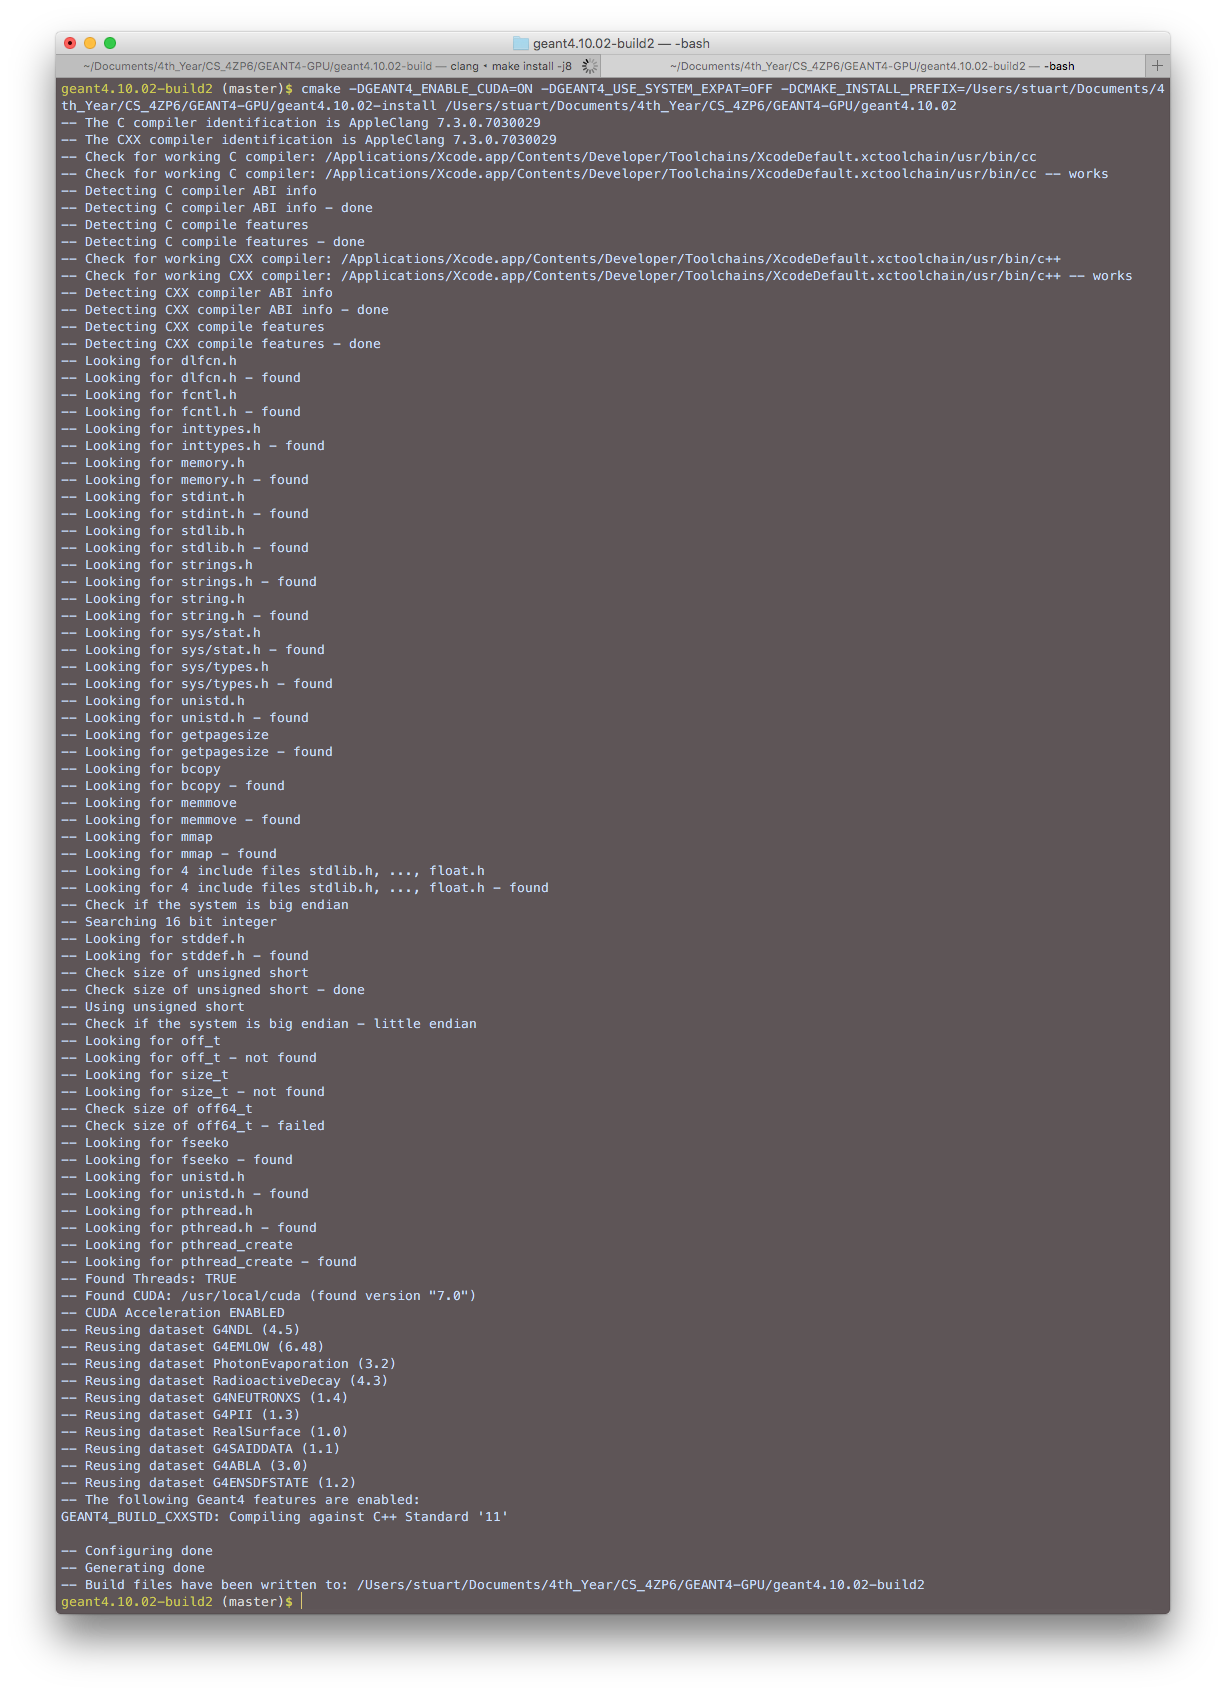
\includegraphics[height=\textheight]{cmakeoutput.png}
\end{figure}

\item Once the previous step is completed, all the makefiles required to build GEANT4-GPU are generated, all dependencies are installed, and all that remains is to actually compile Geant4.\\

In your shell navigate to the \texttt{geant4.10.02-build} directory created in step \ref{StepMkdir} and run the following command:
\texttt{make install}\\

This step can take several hours depending on the speed of your computer.
\item GEANT4-GPU is now installed and ready to be used with your simulations. For more information on creating simulations, see section \ref{SecSimulations}. If you encountered any errors, refer to section \ref{SecTroubleshooting}.
\end{enumerate}

\subsubsection{Installing on McMaster's GPU Servers}\label{SecMac}
If installing GEANT4-GPU on McMaster's GPU servers, the instructions above can be followed with minor differences:
\begin{itemize}
\item The default gcc compiler on the servers is too old to build Geant4, so add the following command to your \texttt{.bash\_profile} to use a newer version:\\
\texttt{. /opt/rh/devtoolset-3/enable}
\item In step \ref{StepCMake}, add the following flag to the CMake command:\\
\texttt{-DCUDA\_HOST\_COMPILER=/usr/bin/g++}. This compiles CUDA with the older version of gcc that's installed on the server, as the latest version is not supported.
\end{itemize}

\section{Execution} % Stuart
Geant4 is not an executable program in the traditional sense. It is instead a large set of libraries, designed to work together and that give you, the user, a framework to develop simulations for your work. The development of such simulations is not within the scope of this manual, but it is well-documented with a thorough guide available at \url{http://Geant4.web.cern.ch/Geant4/UserDocumentation/UsersGuides/ForApplicationDeveloper/html/index.html}.\\

This section will instead outline how one would go about using (or not using) CUDA computations with an existing simulation. The \texttt{Hadr04} example that comes with Geant4 will be used as the simulation to demonstrate this.


\subsection{Enabling/Disabling CUDA} % Stuart
\begin{figure}[!hbtp]
\centering
\caption{Results of CMake command to disable CUDA}\label{FigDisable}
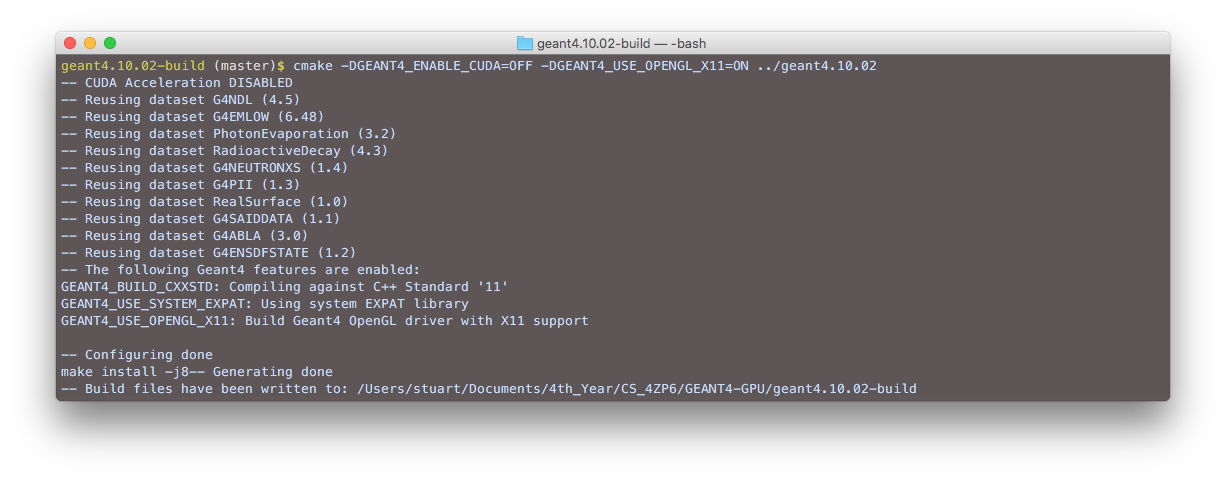
\includegraphics[width=0.9\textwidth]{cmakedisable.png}
\end{figure}

The installation guide details how to build the Geant4 libraries that will be used by your simulation. The CMake command from step \ref{StepCMake} includes a flag that determines whether or not CUDA will be used -- \texttt{-DGEANT4\_ENABLE\_CUDA=ON}. Changing this value to \texttt{OFF} will cause Geant4 to build without any CUDA features, and without requiring \texttt{nvcc}, the CUDA compiler. After step \ref{StepCMake} finishes, users will have to rebuild Geant4 by executing the \texttt{make install} command from their \texttt{geant4.10.02-build} directory. To re-enable CUDA, simply change the value to \texttt{ON} and rebuild again.


\subsection{Building the Simulation}\label{SecSimulations} % Stuart
After Geant4 has been built, building the simulation is very straightforward. First, navigate to your simulation's root folder (\texttt{geant4.10.02/examples/hadronic/Hadr04} in our case) in your terminal. Then, create a new directory \texttt{bin}, so your Hadr04 folder now has two folders, \texttt{bin} and \texttt{src}. Go into the \texttt{bin} folder and run \texttt{cmake ../src} followed by \texttt{make}. That's it!

\subsection{Running the Simulation}\label{SecRedirect} % Stuart
There are two main methods of running a Geant4 simulation. The first is to simply run the executable, in our case by running \texttt{./Hadr04} in the Hadr04 directory. This launches an interactive Geant4 command prompt, and you can manipulate all aspects of the simulation from within it, including the types of particles, their number, and their energies. This also allows you to visualize the simulation using the \texttt{vis} commands.\\

\begin{figure}[!hbtp]
\centering
\caption{\texttt{Hadr04} Example with Visualization}\label{FigVis}
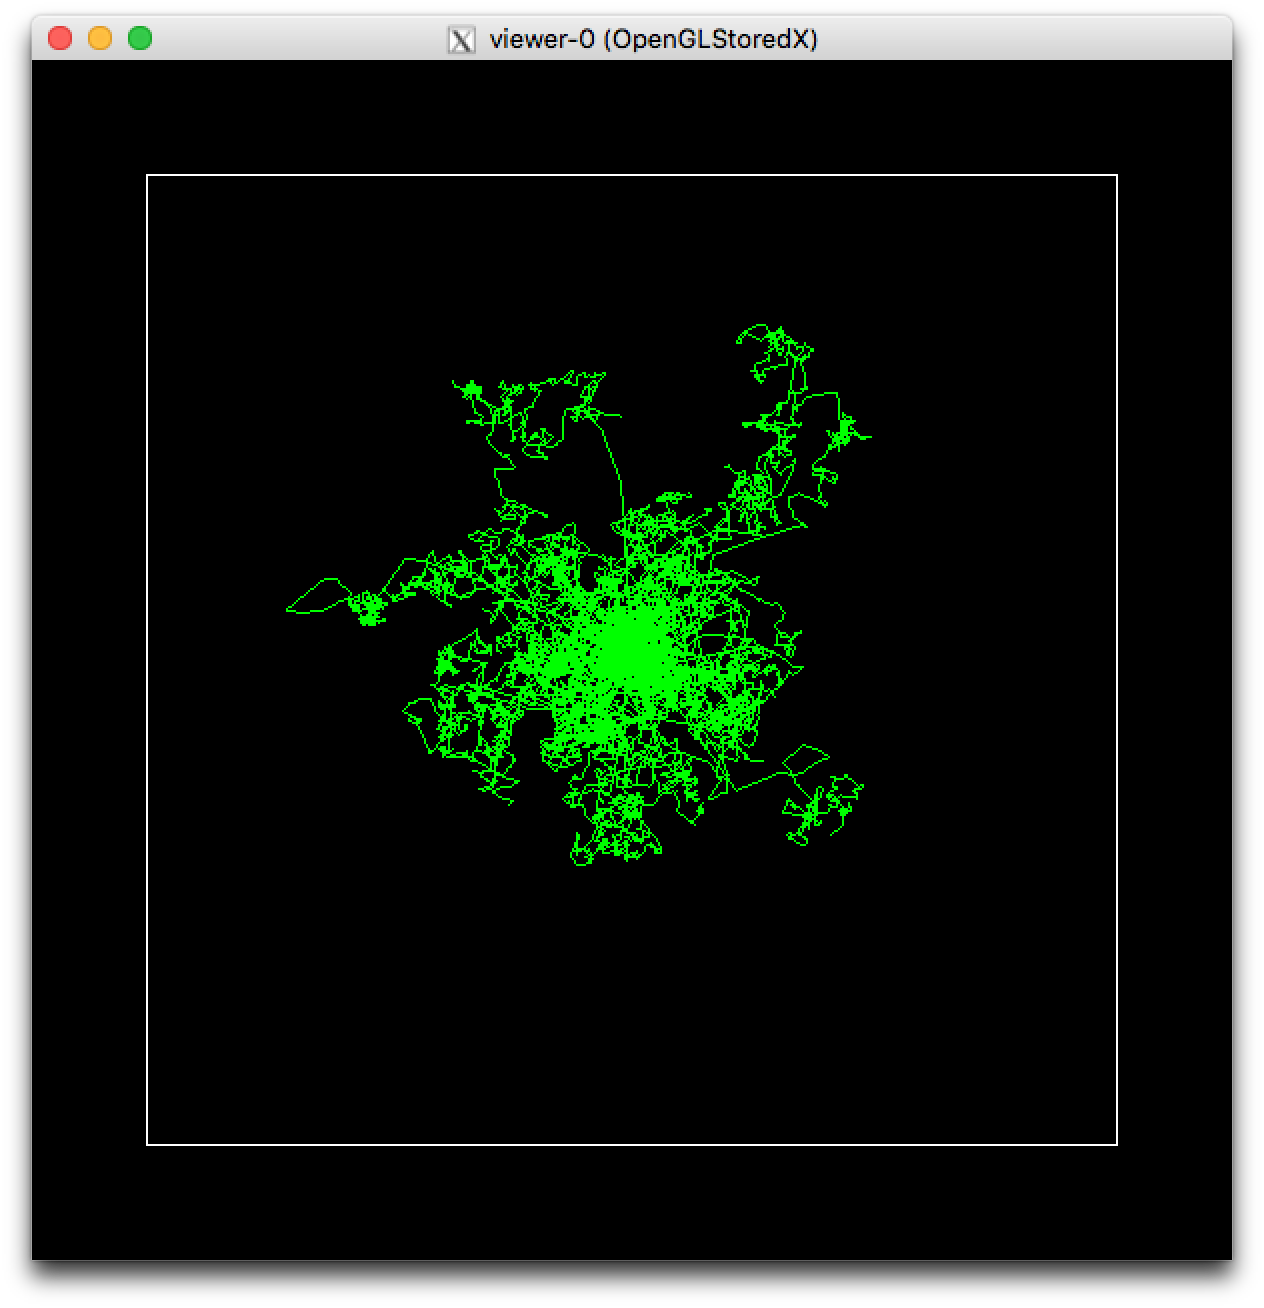
\includegraphics[width=0.5\textwidth]{hadr04_vis.png}
\end{figure}

The alternative is to create a macro file that contains a sequence of commands that would be manually given to the interactive prompt, making it much easier to run a given simulation more than once and without requiring user interaction. Both methods print the results of the simulation out to the terminal window, as well as the running time of the simulation. If you wish to save the results to a file, that can easily be done via redirection in Unix. For example, if you wish to save the results of your simulation using \texttt{myMacro.mac} to \texttt{results.txt}, simply run \texttt{./Hadr04 myMacro.mac > results.txt}.

\section{Porting Other Geant4 Modules to CUDA} \label{SecDev} % Stuart
There is currently one class in GEANT4-GPU that uses CUDA -- \texttt{G4ParticleHPVector}. This class was originally chosen as it was thought to be well-suited to parallelism. Although certain functions within the class are, the majority of the time spent within the class is not in these functions, the main reason for the performance degradations when CUDA is enabled.\\

There is indeed the possibility that there are other classes within Geant4 that are better suited to parallelism. This section will outline the general methodology we used to port \texttt{G4ParticleHPVector} with the hopes that it may be of use to future developers or users.

\subsection{Layout of Source Files} % Stuart
An important consideration during development was to keep the CUDA code separate from the main Geant4 codebase as much as possible. A directory was created named \texttt{cuda} in \texttt{geant4.10.02/source/externals} to contain all CUDA source code. The \texttt{cuda} folder contains two folders, \texttt{include} and \texttt{src}, as well as the CMakeLists.txt file with the CUDA compilation directives. All header files are in \texttt{include}, and the CUDA source files are in \texttt{src}.

\subsection{CMake Changes} % Stuart
Geant4 uses CMake as its build system, and minor modifications need to be made to integrate with CUDA. This consists of adding a variable at the top level CMakeLists file to enable or disable CUDA, and creating a {Geant4\_Add\_Library\_Cuda} macro to Geant4MacroLibraryTargets. This makes use of the \texttt{cuda\_add\_library} function included in CMake. More details can be found in the project's detailed design document.

\subsection{Interfacing with Existing Code} % Stuart
We used compiler directives within the default G4ParticleHPVector.cc file to make use of the CUDA code or to use the original implementation based on the flag passed to Geant4 during the build phase. If the flag is true, an object of type \\\texttt{G4ParticleHPVector\_CUDA} is initialized and all function calls become one line calls to the corresponding function on the G4ParticleHPVector\_CUDA object. For example, the \texttt{GetY} function looks like the following:
\begin{lstlisting}
G4double GetY(int i) {
	#if GEANT4_ENABLE_CUDA
		return cudaVector->GetY();
	#else
		< existing code from G4ParticleHPVector.cc >
	#endif
}
\end{lstlisting}

\subsection{Naming Conventions} % Stuart
It is important to use naming conventions to ensure clarity within a project that contains many possible ambiguities. The two main conventions used were adding a ``\_CUDA" suffix to all source files within the \texttt{cuda} directory as well as to the class name of any classes implemented in CUDA. In addition to this, within all CUDA files there are two main types of pointer -- those to GPU memory and those to CPU memory. To distinguish between these, all pointers to main memory are prepended with ``h\_''(for host) and pointers to GPU memory with a ``d\_''(for device).

\section{Troubleshooting}\label{SecTroubleshooting} % Matt
\subsection{Installation} % Matt
\begin{itemize}
\item Ensure path names are correct in step \ref{StepCMake} of installation
\item The paths in step \ref{StepCMake} of installing Geant4 paths must be absolute, relative paths will not work
\item Spaces in path names may cause issues on some systems
\end{itemize}

\subsection{Running the Simulation} % Matt 
\begin{itemize}
\item Ensure that your graphics card meets the requirements detailed in section \ref{SecCardReqs}
\end{itemize}

\subsection{FAQ} % Matt
\subsubsection{What is Geant4?}\label{SecBackground}
Many physics researchers use Geant4 to learn about how particles interact with a specific environment. It is a toolkit (i.e. a set of libraries) that uses the Monte Carlo model, meaning each particle's properties are calculated independently according to certain probabilities. Users develop simulations based on these libraries.

\subsubsection{How will a GPU improve the performance?}
GPU's contain a large amount of cores that can perform calculations much more quickly than a CPU if the problem is well-suited to parallelization. Geant4 runs relatively simple calculations on millions of particles, and each particle is completely independent of the others. This is exactly that sort of well-suited problem, and stands to see large performance gains.

\subsubsection{Where can I find more information about Geant4?}
For more information, check out the official website at \url{http://Geant4.web.cern.ch/Geant4/}.

\subsubsection{Helpful Pages}
\begin{itemize}
\item Download page for Geant4 source code: \url{http://Geant4.web.cern.ch/Geant4/support/download.shtml}
\item Getting Started guide: \url{http://Geant4.web.cern.ch/Geant4/support/gettingstarted.shtml}
\item Installation Guide for Geant4 (does not include CUDA): \url{http://Geant4.web.cern.ch/Geant4/UserDocumentation/UsersGuides/InstallationGuide/html/index.html}
\end{itemize}

\section{Precautions and Warnings}
By default when running a simulation all output is displayed in the Terminal window. This means that closing the terminal window after a simulation completes will lose all the results. To prevent this, it is recommended to redirect the output to a file, as described in section \ref{SecRedirect}.

\end{document}
